\chapter{Introducción}\label{cap1}
\section{Los problemas clásicos de levantamiento: extensión y clasificación}\label{sec:levext}
En distintos contextos matemáticos encontramos dos problemas básicos, común a todos ellos, si los despojamos de las características propias de un entorno: los problemas de extensión y levantamiento. \par

\subsection*{El problema de la extensión}\label{c1:ext}
Dado un diagrama de aplicaciones continuas 
$$
\begin{tikzcd}
	A \rar{f} \dar[hook]{i} & Y \\
	X \urar[dashed]{\tilde{f}}	&
\end{tikzcd} 
$$
donde $i$ es una ``inclusión'' en un contexto dado, ¿cuándo existe $\tilde{f}$, extensión de $f$? \par

La respuesta no es trivial. Es claro que, incluso si $i$ no es inclusión, ha de verificarse que si $i(a)= i(b)$ entonces $f(a) = f(b)$. Pero incluso si $i$ es biyectiva es necesario exigirle a $X$, para que la única $\tilde{f}$ posible sea continua, que posea la topología de la identificación determinada por $i$: 
$$
\theta \subset X \text{ es abierto si y sólo si } i^{-1} (\theta) \text{ es abierto de } A. 
$$
\newpage
Hay varios ejemplos de resultados que dan respuesta a este problema. Algunos dan una respuesta positiva:
\begin{teor} 
Si $X,Y$ son espacios métricos, $Y$ completo, y $A$ es denso en $X$, toda aplicación uniformemente continua $f:A\longrightarrow Y $ se extiende a una uniformemente continua $\tilde{f} : X \rightarrow Y$.
\end{teor} 

\begin{teor}[de Extensión de Tietze]
Sea $X$ normal, $A \subset X$ cerrado, $I \subset \mathbb{R}$ intervalo. Entonces toda $f : A \rightarrow I $  admite una extensión $\tilde{f} : X \rightarrow I$.
\end{teor}
\hypertarget{c1t:retractoh}{Mientras que la de otros es negativa:}
\begin{teor} \label{c1t:retracto}
La esfera $S^{n}$ no es un retracto del disco $D^{n+1}$. En otras palabras, la identidad $S^{n} \rightarrow S^{n}$ no se extiende a $D^{n+1}$.
\end{teor}

\subsection*{El problema del levantamiento}\label{c1:lev}
Dualmente \footnote{Dual en el sentido de ``Eckmann-Hilton'', dualidad que se definirá más adelante.},
nos encontramos con el problema del levantamiento de aplicaciones continuas. Es el siguiente: dado un diagrama
$$
\begin{tikzcd}
	{}	& X \dar[two heads]{p} \\
	Y \urar[dashed]{\tilde{f}} \rar{f} & B
\end{tikzcd}
$$
donde $p$ es sobreyectiva ¿cuándo existe $\tilde{f}$, levantamiento de $f$?\\ 
La respuesta tampoco es elemental. Incluso si $p$ es biyectiva hay que exigirle que sea homeomorfismo para que la única $\tilde{f}$ sea continua.\par

Igualmente hay resultados clásicos en distintos ambientes que contestan parcialmente esta cuestión.

\begin{teor} 
Sea $A \subset \mathbb{R}^2$ un conjunto estrellado respecto a $x_{0} \in A$ y $f : A \longrightarrow S^{1}$ una aplicación continua. Entonces f queda determinada de forma continua por su función angular, esto es, existe una aplicación $\tilde{f} : A \longrightarrow \mathbb{R}$ de tal forma que el siguiente diagrama es conmutativo:
$$
\begin{tikzcd}
	{}	& \mathbb{R} \dar{exp} \\
	A \urar{\tilde{f}} \rar{f} & S^1
\end{tikzcd}
$$
Esto es, $f(x) = (cos\tilde{f}(x), sen\tilde{f}(x))$. Es más, dos tales funciones $\tilde{f}$ se diferencian en un múltiplo entero de $2\pi$.
\end{teor}

Estos problemas son, en parte, origen de la teoria de homotopía. Muchas veces, los problemas de extensión y levantamiento son puramente homotópicos: \par
\begin{quotation}
Hay aplicaciones $p : X \longrightarrow B$ para las que existe el levantamiento de $f : \nobreak Y \longrightarrow B$ si existe el levantamiento de una ``deformada'' de $f$. \\
De igual forma existen algunas aplicaciones $i : A \longrightarrow X$ para las que existe una extensión de $g : A \longrightarrow Y$ si y sólo si existe alguna extensión para una ``deformada'' de g.
\end{quotation}
Introduzcamos el concepto de deformación en homotopía:
\begin{defin}
Dos aplicaciones $f, g : X \longrightarrow Y$ se dicen homótopas (deformables la una en la otra), denotado por $f \simeq g$, si existe  $H : X \times [0,1] \longrightarrow Y$ una aplicación tal que $H(x ,0) = f(x)$ y $H(x, 1) = g(x)$.
\end{defin}
Llegados a este punto, los problemas de extensión y levantamiento deparan ahora a un problema común de clasificación. ¿Cuándo dos aplicaciones $X \longrightarrow Y$ son homótopas? ¿Cómo es el conjunto $[X, Y]$ de clases de homotopía de aplicaciones $X \longrightarrow Y$? \par 
Los métodos que se siguen son, a grosso modo, de dos enfoques distintos:\\
Por una parte, a los espacios se le asocian modelos algebraicos y morfismos entre los respectivos modelos algebraicos a las aplicaciones. Estas asociaciones permiten parcialmente su clasificación. \par 
Como ejemplo, probemos el \hyperlink{c1t:retractoh}{teorema anterior} por el que $S^n$ no es un retracto de $D^{n+1}$. Para ello, asociemos a $S^n$ un invariante algebraico no nulo (como por ejemplo el grupo de homología $n$-ésimo). Como el disco $D^{n+1}$ es deformable a un punto, todos esos invariantes se hacen 0. Si $S^n$ fuese retracto de $D^{n+1}$ existiría un diagrama como el siguiente:
$$
\begin{tikzcd}
	S^n \arrow{rr}{Id_{S^n}} \drar{i} & & S^n \\
		&	D^{n+1} \urar{r} & 
\end{tikzcd}
$$
que algebraicamente daría lugar a 
$$
\begin{tikzcd}
	0 \neq F(S^n) \arrow{rr}{Id} \drar & &  F(S^n) \neq 0 \\
		&	0 \urar & 
\end{tikzcd}
$$
lo que resulta contradictorio. \par

Por otra parte, para saber más sobre $[X, Y]$ es habitual tratar de dotar a este conjunto de otras estructuras (grupo, módulo...) que den luz sobre su comportamiento. \par
\section{Homotopía: Nociones básicas}\label{sec:homotbas}
La relación de homotopía es básica y formaliza la noción de deformación continua de dos espacios: dos aplicaciones $f, g : X\longrightarrow Y$ son homótopas si existe $H : X \times I \longrightarrow Y$ tal que $H(x, 0) = f(x)$, $H(x, 1) = g(x)$. 
\begin{prop}
La relación de homotopía es una relación de equivalencia en el conjunto de aplicaciones continuas de $X$ a $Y$.
\end{prop}
\begin{demo} 
La propiedad reflexiva es clara sin más que tomar la aplicación $F(x,t) = x$.\\
Para la simétrica, si $H : f \simeq g$ entonces $F : X \times I \longrightarrow Y$, $F(x, t) = H(x, 1-t)$ es una homotopía de $g$ a $f$.\\
Veamos ahora la transitiva. Si $F : f \simeq g$, $H : g \simeq h$ entonces $G : X \times I \longrightarrow Y$,

$$G(x, t) = 
\begin{cases}
	F(x, 2t) 	& 	\text{ si } t \leq \frac{1}{2}\\
	H(x, 2t - 1)& 	\text{ si } t \geq \frac{1}{2}
\end{cases}$$ 
es una homotopía de $f$ a $h$.
\end{demo}
\begin{ejems}
\begin{enumerate}
\item \label{ej1:1} Cuando $X = I$, esto es, al trabajar con curvas, se observa mejor la deformación:
\begin{figure}[h]
\centering
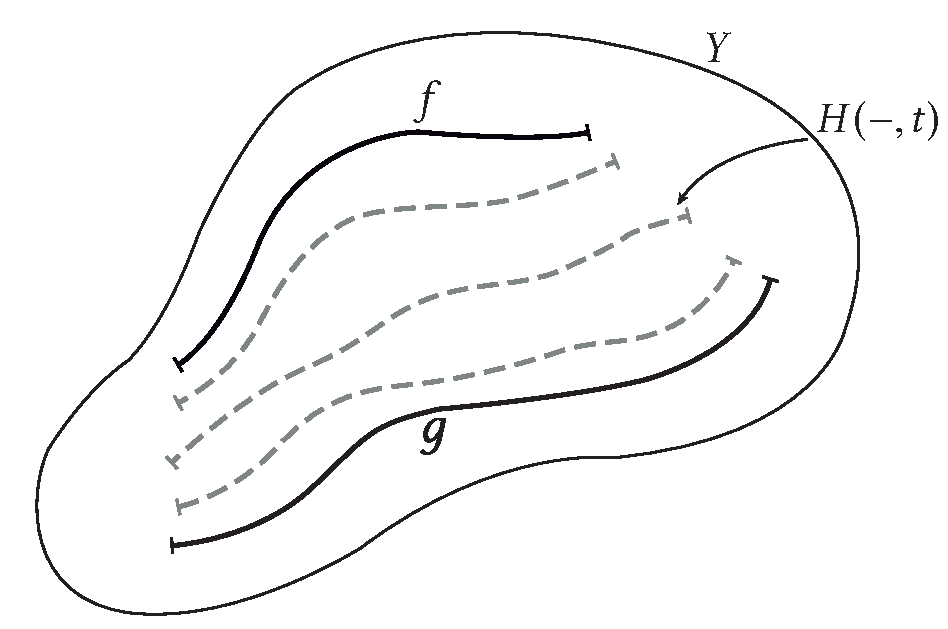
\includegraphics[width=0.4\textwidth]{images/homotcamin.pdf}
\end{figure}
\item \label{ej1:2} Sean $X = Y = \mathbb{R}^n$, y consideremos las aplicaciones $f = Id_{\mathbb{R}^n}$ y $g \equiv 0$. Entonces $f \simeq g$ mediante la aplicación
$$H : \mathbb{R}^n \times I \longrightarrow \mathbb{R}^n$$ $$H(x, t) = tx$$
\end{enumerate}
\end{ejems}
A menudo estamos interesados en aplicaciones entre pares
$$f : (X, A) \longrightarrow (Y, B)$$ que no es más que una aplicación continua tal que $f(A) \subset B$. En este caso, $f, g : (X, A) \longrightarrow (Y, B)$ son homótopas si existe $H : X \times I \longrightarrow Y$ tal que $\forall t \in I$, $H_t = \nobreak H(-, t) : (X, A) \longrightarrow (Y, B)$.\par
Un caso particular de suma importancia es el de los espacios punteados $(X, x_0)$. En este caso, $f \simeq g : (X, x_0) \longrightarrow (Y, y_0)$ si existe $H: X \times I \longrightarrow Y$ tal que $H(x, 0) = f(x), H(x, 1) = g(x)$ y $H(x_0, t) = y_0$ $\forall t \in I$.\\
\begin{ejems}
\begin{enumerate}
\item \label{ej2:1} En el ejemplo anterior \ref{ej1:2}, podemos considerar $f \simeq g : (\mathbb{R}^n, 0) \longrightarrow (\mathbb{R}^n, 0)$ tomando como homotopía la misma función $H$.

\item \label{ej2:2} Si consideramos un espacio como el siguiente: \\
\begin{tabular}{ll}
\begin{minipage}{0.5\textwidth}
Tenemos que $f : I \longrightarrow Y$ es obviamente homótopa a la constante en $y_0$ que denominamos $c_{y_0}$. Pero la aplicación de pares $f : (I, \{ 0,1 \}) \longrightarrow (Y, y_0)$ no es homótopa a la constante $c_{y_0}$.
\end{minipage}
&
\begin{minipage}{0.5\textwidth}
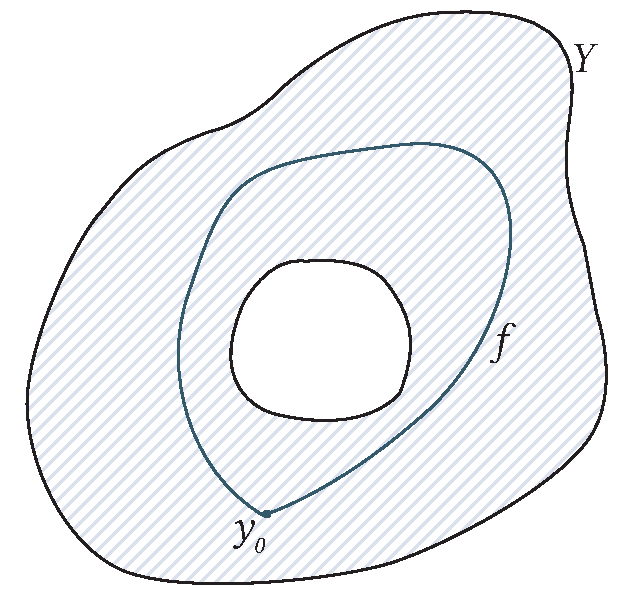
\includegraphics[width=0.65\textwidth]{images/homotrelatalt.pdf}
\end{minipage}
\end{tabular}

\item \label{ej2:3} Dado $E^2 = \{ x \in \mathbb{R}^2 : \| x \| \leq 1 \}$, tenemos que $Id \simeq a$ donde $a$ es la función antípoda mediante la hopotopía de la rotación: $H : E^2 \times I \longrightarrow E^2$ dada por $H(x, t) = H(\rho e^{i\theta}, t) = \rho e^{i(\theta + t\pi)}$ \par
\begin{figure}[h]
\centering
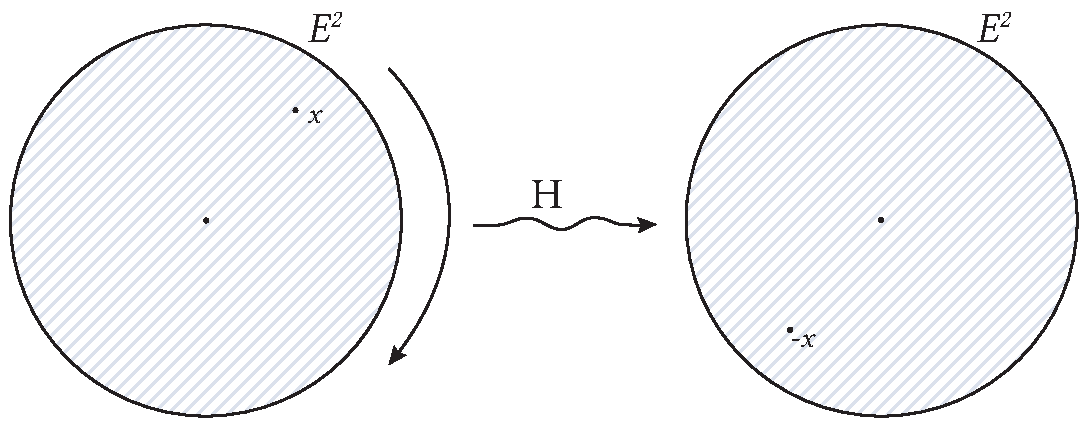
\includegraphics[width=0.65\linewidth]{images/homotrotacalt.pdf}
\end{figure}
Es más, como aplicaciones de pares, $Id \simeq a$ mediante $H : (E^2, S^1) \times I \longrightarrow (E^2, S^1)$. Sin embargo, $\nexists \, x_0 \neq 0$ tal que $Id \simeq a$ como aplicaciones $(E^2, x_0) \longrightarrow (E^2, -x_0)$.
\end{enumerate}
\end{ejems}
Al conjunto cociente formado por las clases de homotopía de aplicaciones continuas de $(X, A)$ en $(Y, B)$ se le denota por $[(X, A), (Y, B)]$.\\
Por tanto, ya podemos definir nuestros ``objetos deformables''.
\begin{defin}
Dos espacios $X$ e $Y$ son homotópicamente equivalentes si existen aplicaciones $f: X \longrightarrow Y$ y $g: Y \longrightarrow X$ tales que $g \circ f \simeq 1_X$ y $f \circ g \simeq 1_Y$. A las aplicaciones $f$ y $g$ se les denomina equivalencias de homotopía.
\end{defin}

\begin{ejems}
\begin{enumerate}
\item \label{ej3:ret} \textbf{Retractos}: 
\begin{tikzcd}
A \rar[hook]{i} & X  
\end{tikzcd}
es un retracto de X si existe una aplicación $r : X \longrightarrow A$ tal que $r \circ i = 1_A$.
Decimos que $A$ es un retracto de deformación de $X$ si además $i \circ r \simeq 1_X$.\\
Como ejemplo, $S^n = \{ x \in \mathbb{R}^{n+1}$ : $\| x \| = 1 \}$ es un retracto de deformación de $\mathbb{R}^{n+1} -\{ 0 \}$. En efecto, si consideramos 
\begin{align*}
r : \mathbb{R}^{n+1} &-\{ 0 \} \longrightarrow S^n \\
x &\longmapsto \frac{x}{\| x \|}
\end{align*}
entonces 
\begin{align*}
H : \mathbb{R}^{n+1} &-\{ 0 \} \times I \longrightarrow \mathbb{R}^{n+1} -\{ 0 \} \\
H(x, t) &= (1 - t)x + \frac{tx}{\| x \|} 
\end{align*}
es una homotopía entre $Id_{\mathbb{R}^{n+1} -\{ 0 \}}$ e $i \circ r$.

\item \label{ej3:contr} \textbf{Espacios contráctiles}: Un espacio X es contráctil si tiene el mismo tipo de homotopía de un punto, o equivalentemente, la identidad en $X$ es homótopa a una constante, o un punto es retracto de deformación del espacio. Antes hemos visto que $\mathbb{R}^n \simeq \ast \simeq D^n $.

\item \label{ej3:peine} \textbf{El espacio peine} P es un espacio contráctil. P es el conjunto definido de la siguiente forma: 

\begin{tabular}{ll}
\begin{minipage}{0.3\textwidth}
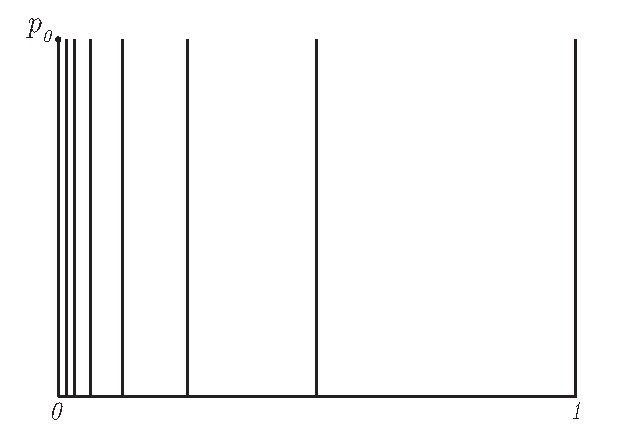
\includegraphics[width=\textwidth]{images/peine.pdf}
\end{minipage}
&
\begin{minipage}{0.6\textwidth}
\[ P = \bigcup_{n=1}^\infty \left( \left\lbrace \frac{1}{n} \right\rbrace \times [0, 1]\right) \cup \{ 0 \} \times [0, 1] \cup [0, 1] \times \{ 0 \} \]
que obviamente es contráctil, aunque $Id_P \not \simeq_{p_0} c_{p_0}$ para un $p_0 \notin [0, 1] \times \nobreak \{ 0 \} $.
\end{minipage}
\end{tabular}
\end{enumerate}

\end{ejems}
Relacionado con el ejemplo \ref{ej3:contr} y con el problema de la extensión tenemos el siguiente resultado:\\
\begin{teor}
Sea $f : S^n \longrightarrow X$ una aplicación continua. Entonces $f \simeq \ast$ si y sólo si $f$ se extiende al disco. 
\[
\begin{tikzcd}
	S^n \arrow{rr}{f} \drar[hook] & & X \\
		& D^{n+1} \urar{\tilde{f}}
\end{tikzcd}
\]
\end{teor}
\begin{demo}
Supongamos $H : f \simeq c_{x_0}$. Definimos entonces $\tilde{f} : E^{n+1} \longrightarrow X$ dada por:
\[
\tilde{f}(p )= 
\begin{cases}
	x_0 & \text{ si }\| p \| \leq \frac{1}{2} \\
	H(\frac{p}{\| p \|}, 2 - 2\| p \|) & \text{ si } \| p \| \geq \frac{1}{2}
\end{cases}
\]
que es la extensión que queríamos.

Recíprocamente, si $\tilde{f}$ es una extensión, $H(x, t) = \tilde{f}((1 - t)x)$ es una homotopía de $f$ a la constante. 
\end{demo}

\subsection{Espacios comúnmente utilizados}\label{c1:espcomun}
Algunas de las construcciones que serán de utilidad son las siguientes:
\begin{itemize}
\item \hypertarget{ecom:prod}{\textbf{El producto de espacios}} $X \times Y$ \\

\item \hypertarget{ecom:suma}{\textbf{La suma puntual}} o ``wedge'', denotado por $X \vee Y$ que puede verse como el conjunto cociente $X \dot\cup Y \Bign/ x_0 \sim \nobreak y_0$ o como un subconjunto de  $X \times Y$, esto es, $X \vee Y = X \times \{y_0\} \cup \{x_0\} \times Y$\\

\item \hypertarget{ecom:smash}{\textbf{El smash}} definido como $X \wedge Y = X \times Y \Bign/ X \vee Y$. Esto es, el producto en el que identificamos ``los ejes'' a un punto.\\


\begin{tabular}{ll}
\begin{minipage}{0.5\textwidth}
\item \hypertarget{ecom:cono}{\textbf{El cono de $X$.}} Dado $X$, el cono de $X$ se define como $CX = \faktor{X \times I}{X \times \{0\}}$.\\
Si queremos ``puntearlo'', hacemos además
\[CX = \faktor{X \times I}{X \times \{ 0 \} \cup \{ x_0 \} \times I} \] 
\end{minipage}
&
\begin{minipage}{0.5\textwidth}
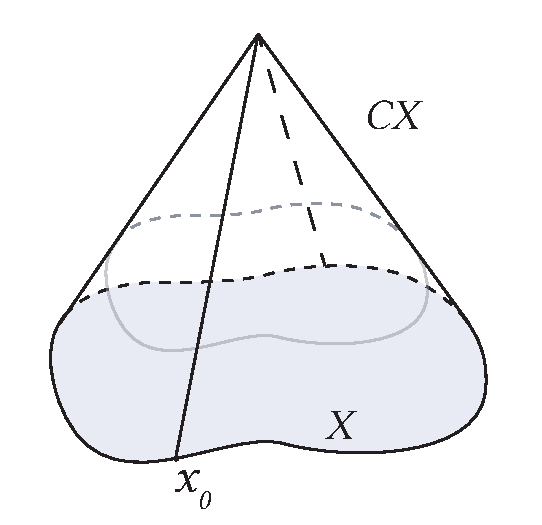
\includegraphics[width=0.6\textwidth]{images/conox.pdf}
\end{minipage}
\end{tabular}
 
 y el punto base es $[x_0, t]$. Claramente la aplicación 
\begin{align*}
X &\longhookrightarrow CX \\ 
x &\longmapsto [(x, 1)]
\end{align*}
es un homeomorfismo en su imagen por lo que podemos pensar en $X$ como un subespacio del cono. Además $CX$ es contráctil.
\end{itemize}
\subsection{Adjuntando celdas o cómo pegar un disco a un espacio}\label{c1:unionceldas}
Sea $X$ un espacio topológico y $E^n$ un disco de dimensión $n \geq 1$. \\
 Sea $f : S^{n-1} \longrightarrow X$ una aplicación continua. Definimos $X \cup_f e^n$, el espacio obtenido adjuntando a X una $n$-celda mediante $f$: \par
\begin{tabular}{ll}
\begin{minipage}{0.5\textwidth}
\[ X \cup_f e^n := \faktor{ X \dot{\cup} E^n}{ \sim} \]
\end{minipage}
&
\begin{minipage}{0.5\textwidth}
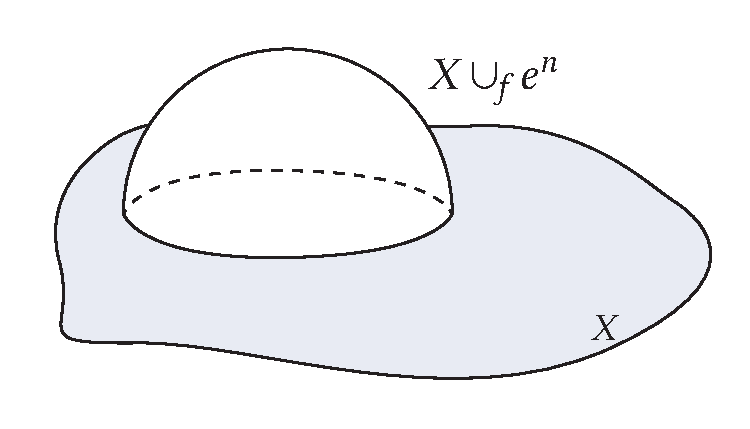
\includegraphics[width=0.8\textwidth]{images/uceldas.pdf}
\end{minipage}
\end{tabular}


donde $\sim$ es la menor relación de equivalencia que contiene a $x \in S^{n-1} \sim f(x)$\\

\begin{prop}
La adjunción de una celda sólo depende del tipo de homotopía de la aplicación de adjunción.
\end{prop}
\begin{demo}
Sean $f ,g : S^{n-1} \longrightarrow X$ dos funciones con el mismo tipo de homotopía, $f \simeq g$. Veamos que entonces que $X \cup_f e^n \simeq X \cup_g e^n$.\par 
Si $H : f \simeq g$, definimos las siguientes funciones:
$$k : X \cup_f e^n \longrightarrow X \cup_g e^n
\text{ dada por }
k(x) = 
\begin{cases}
	x  & \text{si } x \in X \\
	2x & \text{si } x \in e^n$, $\| x \| \leq \frac{1}{2} \\
	H(\frac{x}{\| x \|}, 2 - 2\|x\|) & \text{si } \| x \| \geq \frac{1}{2}
\end{cases}$$ 
$$h : X\cup_g e^n \longrightarrow X \cup_f e^n
\text{ dada por }
h(x) = 
\begin{cases}
	x  & \text{si } x \in X \\
	2x & \text{si } x \in e^n$, $ \| x \| \leq \frac{1}{2} \\
	H(\frac{x}{\| x \|}, 2\| x \| - 1 & \text{si } \| x \| \geq \frac{1}{2}\\
\end{cases}$$
Y tenemos que $h \circ k \simeq 1_{X \cup_f e^n}$ mediante la función $F : X \cup_f e^n \times I \longrightarrow X \cup_f e^n$ dada por: \\
\begin{center}
$F(x,t) = 
\begin{cases}
	x  & \text{si } x \in X \\
	4x & \text{si } \| x \| \leq \frac{1}{4} \\
	H(\frac{x}{\| x \|}, (4\|x\| - 1)t) & \text{si } \frac{1}{4} \leq \| x \| \leq \frac{1}{2} \\
	H(\frac{x}{\| x \|}, (2 - 2\|x\|)t) & \text{si } \| x \| \geq \frac{1}{2}
\end{cases}$ \\
\end{center}
De forma análoga se prueba que $k \circ h \simeq 1_{X \cup_g e^n}$.
\end{demo}
\textbf{Consecuencia:} Si $X$ es arcoconexo, $X \cup_f e^1 \simeq X \vee S^1$ y si $f \simeq \ast$, entonces
$X \cup_f e^n \simeq X \vee S^n$. \\


\begin{teor}
Una aplicación $f : (X, x_0) \longrightarrow (Y, y_0)$ es null-homótopa si y sólo si se extiende a $CX$: 
$$
\begin{tikzcd}
	X \arrow{rr}{f} \drar[hook] & & Y \\
	& CX \urar[dashed]{h} & 
\end{tikzcd}
$$
\end{teor}
\begin{demo}
Sea $H : f \simeq c_{y_0}$ una homotopía. Definimos entonces la aplicación $h : CX \longrightarrow Y$, dada por $h([x, t]) = H(x, t)$. Está bien definida, ya que $H(X \times \{ 0 \} \cup \{ x_0 \} \times I) = y_0$ y se extiende a $f$.\par 
Recíprocamente, dada $h : (CX, \ast) \longrightarrow (Y, y_0)$ extensión de $f$, definimos $H: X \times I \longrightarrow Y$ como $H = h \circ \pi$ (donde $\pi: X \times I \longrightarrow CX$ es la proyección canónica) y se tiene que 
$H(x, 0) = y_0$, $H(x, 1) = f(x)$ y $H(x_0, t) = y_0$.
\end{demo}

\section{Dualidad de Eckmann-Hilton}
Este principio de dualidad, en su forma más básica, consiste en la idea de, dado un diagrama para una construcción, invertir el sentido de las flechas de dicho diagrama. \par 
Un ejemplo de esto son las fibraciones y cofibraciones. Estas dos construcciones son duales en el sentido de Eckmann-Hilton. \par
Una fibración $p : E \longrightarrow B$ verifica que posee la HLP, que se representa por el diagrama:
\[
\begin{tikzcd}
X \arrow{rr}{g} \arrow[hook]{dd}{i_o} &  & E \arrow{dd}{p} \\
\\
X \times I \arrow{rr}{G} \arrow[dashed]{uurr}{\widetilde{G}} & & B
\end{tikzcd}
\]
Y una cofibración $i : A \longrightarrow X$ es tal que posee la HEP, que viene dada por el diagrama:
\[
\begin{tikzcd}
	{} 						  & X \drar{i_0} \arrow[bend left]{drr}{f}			   &        					&   \\
	A \urar[hook] \drar{i_0}  &   												   & X \times I \rar[dashed]{F} & Y \\
	   						  & A \times I  \urar[hook] \arrow[bend right]{urr}{G} &   							&
\end{tikzcd}
\]
Éste último diagrama podemos cambiarlo haciendo uso del \textit{currying}, esto es, considerar aplicaciones $X \times I \longrightarrow Y$ como aplicaciones $X \longrightarrow Y^I$. Así, tendríamos que el diagrama queda de la siguiente forma:\[
\begin{tikzcd}
Y & & X \arrow{ll}{f} \arrow[dashed]{ddll}{\widetilde{F}} \\
\\
Y^I \arrow[two heads]{uu}{\pi} & & A \arrow[hook]{uu}{i} \arrow{ll}{G}
\end{tikzcd}
\]
En el cual se ve que el sentido de las flechas es el contrario que en la fibración. \par
Además esto también se observa entre las sucesiones exactas dadas por fibraciones y cofibraciones: \par
Para una cofibración, teníamos la sucesión de Barratt-Puppe:
\[ X \longrightarrow Y \longrightarrow C_f \longrightarrow \Sigma X \longrightarrow \Sigma Y \longrightarrow \Sigma C_f \longrightarrow \Sigma^2 X \longrightarrow \dots \]
Y para las fibraciones teníamos la sucesión dada por la fibra homotópica de una aplicación:
\[ \dots \longrightarrow \Omega^2 Y \longrightarrow \Omega F \longrightarrow \Omega X \longrightarrow \Omega Y \longrightarrow F \longrightarrow X \longrightarrow Y \]